
%(BEGIN_QUESTION)
% Copyright 2010, Tony R. Kuphaldt, released under the Creative Commons Attribution License (v 1.0)
% This means you may do almost anything with this work of mine, so long as you give me proper credit

Suppose this solenoid-controlled valve refuses to move when the operator pushes the switch.  Whether the switch is pressed or unpressed, the control valve remains in the fully-closed (down) position:

$$\includegraphics[width=15.5cm]{i04202x01.eps}$$

Another technician has already measured 475 volts between terminals {\bf H1} and {\bf H4} on the transformer, and 0 volts between terminals {\bf D} and {\bf X1}, in both pushbutton switch positions.  At that point he gave up and left the system for you to troubleshoot.

Identify the likelihood of each specified fault for this system.  Consider each fault one at a time (i.e. no coincidental faults), determining whether or not each fault could independently account for {\it all} measurements and symptoms in this system.

% No blank lines allowed between lines of an \halign structure!
% I use comments (%) instead, so that TeX doesn't choke.

$$\vbox{\offinterlineskip
\halign{\strut
\vrule \quad\hfil # \ \hfil & 
\vrule \quad\hfil # \ \hfil & 
\vrule \quad\hfil # \ \hfil \vrule \cr
\noalign{\hrule}
%
% First row
{\bf Fault} & {\bf Possible} & {\bf Impossible} \cr
%
\noalign{\hrule}
%
% Another row
Fuse F3 blown (failed open) &  &  \cr
%
\noalign{\hrule}
%
% Another row
Solenoid stuck in ``energized'' position &  &  \cr
%
\noalign{\hrule}
%
% Another row
Solenoid stuck in ``de-energized'' position &  &  \cr
%
\noalign{\hrule}
%
% Another row
Solenoid coil failed open &  &  \cr
%
\noalign{\hrule}
%
% Another row
Solenoid coil failed shorted &  &  \cr
%
\noalign{\hrule}
%
% Another row
Silencer plugged &  &  \cr
%
\noalign{\hrule}
%
% Another row
Vent cap plugged &  &  \cr
%
\noalign{\hrule}
%
% Another row
Wire open between terminals A and E &  &  \cr
%
\noalign{\hrule}
%
% Another row
Wire open between terminals C and H &  &  \cr
%
\noalign{\hrule}
%
% Another row
Wire open between terminals K and B &  &  \cr
%
\noalign{\hrule}
%
% Another row
Valve V1 shut &  &  \cr
%
\noalign{\hrule}
%
% Another row
Valve V2 shut &  &  \cr
%
\noalign{\hrule}
} % End of \halign 
}$$ % End of \vbox

Finally, identify the {\it next} diagnostic test or measurement you would make on this system.  Explain how the result(s) of this next test or measurement help further identify the location and/or nature of the fault.

\vskip 20pt \vbox{\hrule \hbox{\strut \vrule{} {\bf Suggestions for Socratic discussion} \vrule} \hrule}

\begin{itemize}
\item{} Describe some of the problem-solving techniques you could (or did) apply to this question, explaining how your techniques translated the problem into something more manageable.
\end{itemize}

\underbar{file i04202}
%(END_QUESTION)





%(BEGIN_ANSWER)

% No blank lines allowed between lines of an \halign structure!
% I use comments (%) instead, so that TeX doesn't choke.

$$\vbox{\offinterlineskip
\halign{\strut
\vrule \quad\hfil # \ \hfil & 
\vrule \quad\hfil # \ \hfil & 
\vrule \quad\hfil # \ \hfil \vrule \cr
\noalign{\hrule}
%
% First row
{\bf Fault} & {\bf Possible} & {\bf Impossible} \cr
%
\noalign{\hrule}
%
% Another row
Fuse F3 blown (failed open) &  & $\surd$ \cr
%
\noalign{\hrule}
%
% Another row
Solenoid stuck in ``energized'' position & $\surd$ &  \cr
%
\noalign{\hrule}
%
% Another row
Solenoid stuck in ``de-energized'' position &  & $\surd$ \cr
%
\noalign{\hrule}
%
% Another row
Solenoid coil failed open &  & $\surd$ \cr
%
\noalign{\hrule}
%
% Another row
Solenoid coil failed shorted &  & $\surd$ \cr
%
\noalign{\hrule}
%
% Another row
Silencer plugged &  & $\surd$ \cr
%
\noalign{\hrule}
%
% Another row
Vent cap plugged &  & $\surd$ \cr
%
\noalign{\hrule}
%
% Another row
Wire open between terminals A and E &  & $\surd$ \cr
%
\noalign{\hrule}
%
% Another row
Wire open between terminals C and H &  & $\surd$ \cr
%
\noalign{\hrule}
%
% Another row
Wire open between terminals K and B &  & $\surd$ \cr
%
\noalign{\hrule}
%
% Another row
Valve V1 shut & $\surd$ &  \cr
%
\noalign{\hrule}
%
% Another row
Valve V2 shut & $\surd$ &  \cr
%
\noalign{\hrule}
} % End of \halign 
}$$ % End of \vbox

A plugged vent on the valve actuator, while in theory capable of limiting the control valve's upward motion, would not prevent any motion at all from occurring when full pressure is applied to the bottom of the diaphragm.  This is why ``Vent cap plugged'' is checked as impossible rather than possible for this scenario.

\vskip 10pt

A good ``next test'' would be to crack the fitting at port ``C'' of the solenoid valve.  If there is pressure, it means the problem must lie past the solenoid (e.g. valve V1 shut, or a problem in the process control valve).  If there is no pressure at that point, either the solenoid valve is stuck in the ``energized'' position or there is a lack of supply pressure to the solenoid.

%(END_ANSWER)





%(BEGIN_NOTES)

\vskip 20pt \vbox{\hrule \hbox{\strut \vrule{} {\bf Virtual Troubleshooting} \vrule} \hrule}

This question is a good candidate for a ``Virtual Troubleshooting'' exercise.  Presenting the diagram to students, you first imagine in your own mind a particular fault in the system.  Then, you present one or more symptoms of that fault (something noticeable by an operator or other user of the system).  Students then propose various diagnostic tests to perform on this system to identify the nature and location of the fault, as though they were technicians trying to troubleshoot the problem.  Your job is to tell them what the result(s) would be for each of the proposed diagnostic tests, documenting those results where all the students can see.

During and after the exercise, it is good to ask students follow-up questions such as:

\begin{itemize}
\item{} What does the result of the last diagnostic test tell you about the fault?
\item{} Suppose the results of the last diagnostic test were different.  What then would that result tell you about the fault?
\item{} Is the last diagnostic test the best one we could do?
\item{} What would be the ideal order of tests, to diagnose the problem in as few steps as possible?
\end{itemize}


%INDEX% Troubleshooting review: electric circuits

%(END_NOTES)


